% Bayesian Spectral Flow Matching — S² study slides
% Compile from this directory:
%   pdflatex sphere_study_slides.tex
%   pdflatex sphere_study_slides.tex   (second pass for TOC)

\documentclass[aspectratio=169,11pt]{beamer}

\usetheme{Madrid}
\usecolortheme{default}
\setbeamertemplate{navigation symbols}{}
\setbeamertemplate{footline}[frame number]

\usepackage{amsmath,amssymb}
\usepackage{booktabs}
\usepackage{graphicx}
\usepackage{hyperref}

\graphicspath{{./}{../molecule/}}

\title{Bayesian Spectral Flow Matching}
\subtitle{Sphere benchmark, neural operators \& molecular FM}
\author{ETH --- Diffusion models project}
\institute{bayesian-spectral-flow-matching}
\date{\today}

\begin{document}

% ---------------------------------------------------------------------------
\begin{frame}
  \titlepage
\end{frame}

\begin{frame}{Outline}
  \tableofcontents
\end{frame}

% ---------------------------------------------------------------------------
\section{Synthetic benchmark dataset}

\begin{frame}{Target distribution on \texorpdfstring{$S^2$}{S2}}
  \textbf{Fully synthetic ground truth} (\texttt{Dataset/sphere.py}) --- each sample is a random field on the sphere with known spectral law.

  \vspace{0.5em}
  \textbf{Pipeline (informal)}
  \begin{enumerate}\setlength{\itemsep}{0.2em}
    \item Draw coefficients $\boldsymbol{\xi} = (\xi_{\ell m})$ in a real spherical-harmonic basis
    \item Form $f(\theta,\phi) = \sum_{\ell m} \xi_{\ell m}\, Y_{\ell m}(\theta,\phi)$ and evaluate on a grid
    \item Vectorize $f$ for FM training ($800$ cells in the main benchmark: $20{\times}40$)
  \end{enumerate}

  \vspace{0.35em}
  Formal sampling equations on the next slide; geodesic \textbf{graph Laplacian} on the same mesh drives our spectral method.
\end{frame}

\begin{frame}{Generative model --- band-limited fields on \texorpdfstring{$S^2$}{S2}}
  \small
  \textbf{Continuous field.}\quad For band-limit $L_{\max}$ and real SH basis $\{Y_{\ell m}\}_{0\le \ell\le L_{\max}}$,
  \[
    f(\theta,\phi) \;=\; \sum_{\ell=0}^{L_{\max}} \sum_{m=-\ell}^{\ell} \xi_{\ell m}\, Y_{\ell m}(\theta,\phi),
    \qquad
    \xi_{\ell m} \stackrel{\text{i.i.d.}}{\sim} \mathcal{N}\bigl(0,\,\sigma_{\ell m}^2\bigr).
  \]

  \textbf{Spectral decay} (smoothness knob $s>0$, code default $s{=}2$):
  \[
    \sigma_{\ell m} \;=\;
    \begin{cases}
      \sqrt{\mathrm{Var}_0} & \ell = 0,\\[0.35em]
      \bigl(\ell(\ell+1)\bigr)^{-s/2} & \ell \ge 1,
    \end{cases}
  \]

  \textbf{Discrete evaluation.}\quad Grid points $\{(\theta_i,\phi_j)\}$, synthesis matrix $Y \in \mathbb{R}^{N_{\mathrm{grid}} \times N_{\mathrm{coeff}}}$,
  \[
    \mathbf{f} \;=\; Y\,\boldsymbol{\xi} \in \mathbb{R}^{N_{\mathrm{grid}}},
    \qquad N_{\mathrm{coeff}} = \sum_{\ell=0}^{L_{\max}} (2\ell+1).
  \]
  \normalsize
\end{frame}

\begin{frame}{Synthetic ground truth --- band-limit}
  \small
  Random targets from \texttt{generate\_coeff} $\rightarrow$ \texttt{build\_synthesis\_matrix}.

  \vspace{0.35em}
  \begin{columns}[c,onlytextwidth]
    \column{0.48\textwidth}
    \centering
    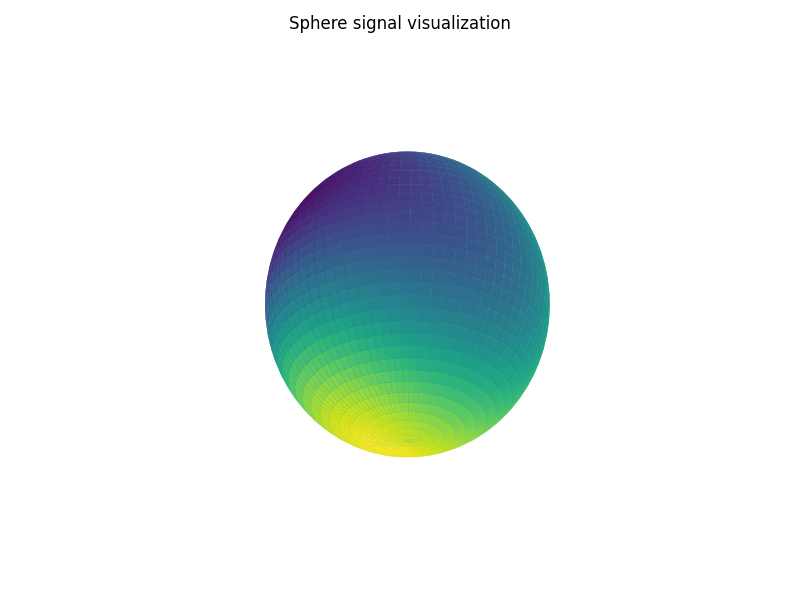
\includegraphics[width=\linewidth,height=0.68\textheight,keepaspectratio]{ground_sohere_L_2.png}\\[0.25em]
    {\small low band-limit $L_{\max}{=}2$}

    \column{0.48\textwidth}
    \centering
    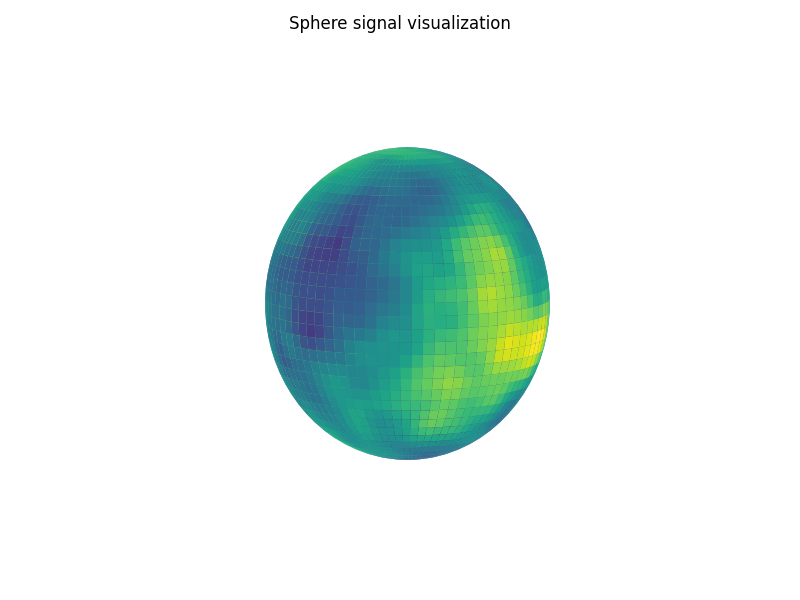
\includegraphics[width=\linewidth,height=0.68\textheight,keepaspectratio]{ground_sohere_L_30.png}\\[0.25em]
    {\small high band-limit $L_{\max}{=}30$}
  \end{columns}

  \vspace{0.3em}
  \footnotesize
  Spectral complexity (harmonic degree) --- swept in later $L_{\max}$ studies.
\end{frame}

\begin{frame}{Synthetic ground truth --- mesh resolution}
  \small
  Same synthesis pipeline; finer $(n_\theta \times n_\phi)$ grids.

  \vspace{0.35em}
  \begin{columns}[c,onlytextwidth]
    \column{0.48\textwidth}
    \centering
    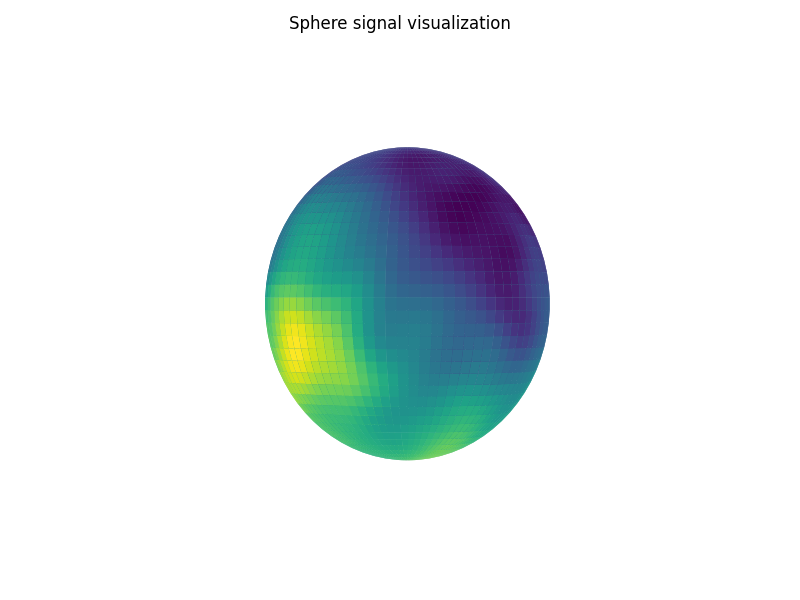
\includegraphics[width=\linewidth,height=0.68\textheight,keepaspectratio]{ground_sohere_40_80.png}\\[0.25em]
    {\small mesh $40{\times}80$}

    \column{0.48\textwidth}
    \centering
    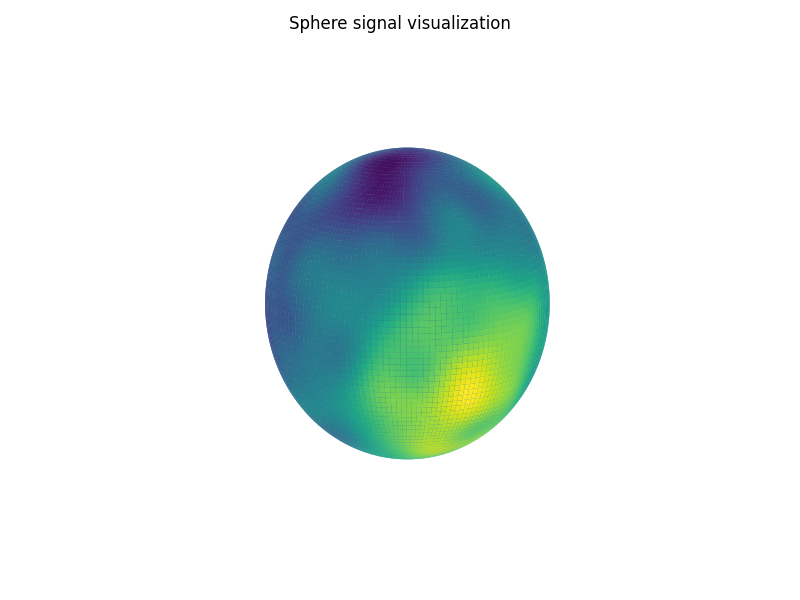
\includegraphics[width=\linewidth,height=0.68\textheight,keepaspectratio]{ground_sohere_80_160.png}\\[0.25em]
    {\small mesh $80{\times}160$}
  \end{columns}

  \vspace{0.3em}
  \footnotesize
  Discretization resolution at fixed $L_{\max}$.
\end{frame}

\begin{frame}{Geodesic graph Laplacian}
  Graph on the same $(n_\theta \times n_\phi)$ grid as the data: nearby cells are connected.

  \vspace{0.6em}
  Edge weights from \textbf{geodesic distance} on $S^2$ and a \textbf{heat kernel}:
  \[
    d_{uv} = \arccos(\mathbf{x}_u \cdot \mathbf{x}_v),
    \qquad
    w_{uv} = \exp\!\left(-\frac{d_{uv}^2}{2\sigma^2}\right).
  \]

  \vspace{0.4em}
  Then $L = D - W$ (standard graph Laplacian).
\end{frame}

% ---------------------------------------------------------------------------
\section{Setting \& method}

\begin{frame}{Goal}
  \textbf{Generative transport} from a source distribution to band-limited random fields on the sphere, evaluated with \textbf{Wasserstein distance} on a fixed grid.

  \vspace{0.6em}
  Compare:
  \begin{itemize}
    \item \textbf{Standard FM} --- Gaussian source, Euclidean OT pairing, MSE flow-matching loss
    \item \textbf{Ours} --- optional \emph{spectral} loss weighting, \emph{Sobolev OT} pairing on the grid Laplacian, \emph{Mat\'ern} source sampling
  \end{itemize}

  \vspace{0.4em}
  Target: coefficients in spherical harmonics up to $L_{\max}$, synthesized on an $(n_\theta \times n_\phi)$ mesh.
\end{frame}

\begin{frame}{Three ablatable components}
  \begin{table}
    \centering
    \small
    \begin{tabular}{@{}llp{5.2cm}@{}}
      \toprule
      \textbf{Flag} & \textbf{Module} & \textbf{Role} \\
      \midrule
      \texttt{use\_spectral} & \texttt{SpectralFM} & Sobolev-weighted CFM loss in Laplacian eigenbasis ($\alpha$) \\
      \texttt{use\_sobolev\_ot} & \texttt{OTDisplacementMap} & Minibatch pairing under Sobolev cost ($\beta$) \\
      \texttt{use\_matern\_source} & Mat\'ern sampler & Source $x_0$ drawn as smooth field on graph ($\nu$, $\tau$) \\
      \bottomrule
    \end{tabular}
  \end{table}

  \vspace{0.5em}
  Sphere benchmark uses geodesic grid Laplacian, SH synthesis matrix $Y$, and Wasserstein metric in \texttt{Tests/metrics.py}.
\end{frame}

% ---------------------------------------------------------------------------
\section{Experiment: component ablation}

\begin{frame}{Experiment --- setup}
  \textbf{3-component ablation} (Wasserstein evaluation on $S^2$)

  \vspace{0.5em}
  \begin{columns}[T,onlytextwidth]
    \column{0.48\textwidth}
    \textbf{Model \& data}
    \begin{itemize}\setlength{\itemsep}{0.15em}
      \item MLP \texttt{intermediate\_dim} = 256
      \item Mesh: $n_\theta{=}20$, $n_\phi{=}40$ $\Rightarrow$ 800 cells
      \item FM steps: 4 \quad Epochs: 1000
      \item $L_{\max} = 5$
    \end{itemize}

    \column{0.48\textwidth}
    \textbf{Hyperparameters}
    \begin{itemize}\setlength{\itemsep}{0.15em}
      \item $\alpha = -1$
      \item $\beta = 2.0$
      \item $\nu = 3.0$, $\tau = 2.0$
    \end{itemize}
  \end{columns}
\end{frame}

\begin{frame}{Experiment --- Wasserstein results}
  \small
  \begin{table}
    \centering
    \begin{tabular}{@{}lc@{}}
      \toprule
      \textbf{Configuration} & \textbf{$W_2$ (lower is better)} \\
      \midrule
      Standard FM & 25.40 \\
      Ours: spectral + Sobolev OT + Mat\'ern (all three) & 8.14 \\
      Ours: Mat\'ern source + spectral loss & \textbf{7.98} \\
      Ours: Mat\'ern source only & 26.14 \\
      Ours: spectral loss only & 25.45 \\
      \bottomrule
    \end{tabular}
  \end{table}

  \vspace{0.5em}
  \textbf{Takeaway:} Enabling all three reaches $W_2 \approx 8.14$ (vs.\ 25.4 baseline). Best run: Mat\'ern + spectral loss ($\approx 7.98$); Sobolev OT adds little on top of that pair. Single components alone stay near baseline.
\end{frame}

\newcommand{\discussionframe}[2]{%
  \begin{frame}{#1 --- discussion}
    \small
    #2
    \normalsize
  \end{frame}%
}

\discussionframe{Experiment --- Wasserstein results}{
  \begin{itemize}
    \item \textbf{Mat\'ern source is the dominant ingredient} --- alone it does not help ($W_2 \approx 26$), but paired with spectral loss it drops to $\approx 8$.
    \item \textbf{Sobolev OT is secondary} on this grid once source and loss are aligned with manifold smoothness.
    \item \textbf{Spectral loss alone} reweights gradients but cannot fix a mismatched Gaussian prior.
  \end{itemize}
}

\newcommand{\exponeviz}[4]{%
  \begin{frame}{Experiment --- #1}
    \vspace{-0.35em}
    \centering
    \includegraphics[width=\linewidth,height=0.82\textheight,keepaspectratio]{#2}\\[0.35em]
    {\small #3 \hfill $W_2 = #4$}
  \end{frame}%
}

\exponeviz{Standard FM}{exp_1_standard.png}{Gaussian source, Euclidean OT, MSE loss}{25.40}
\exponeviz{Ours: all three enabled}{exp_1_all_3.png}{Mat\'ern source + Sobolev OT + spectral loss}{8.14}
\exponeviz{Ours: Mat\'ern + spectral loss}{exp_1_matern_loss.png}{Mat\'ern source + Sobolev-weighted CFM loss}{\textbf{7.98}}
\exponeviz{Ours: Mat\'ern only}{exp_1_matern.png}{Mat\'ern source; standard loss and OT}{26.14}
\exponeviz{Ours: spectral loss only}{exp_1_loss.png}{Sobolev-weighted loss; Gaussian source}{25.45}

\begin{frame}{Open questions}
  \begin{itemize}
    \item Mat\'ern source + spectral loss strongly outperforms Gaussian source --- why?
    \item How should we \textbf{select / calibrate} $(\nu, \tau, \alpha, \beta)$ for a new target?
    \item \textbf{Bayesian update of the source} during training (adaptive prior) --- promising direction?
  \end{itemize}
\end{frame}

% ---------------------------------------------------------------------------
\section{Experiment: \texorpdfstring{$L_{\max}$}{Lmax} sweep}

\begin{frame}{Experiment --- Wasserstein vs.\ \texorpdfstring{$L_{\max}$}{Lmax}}
  \vspace{-0.35em}
  \centering
  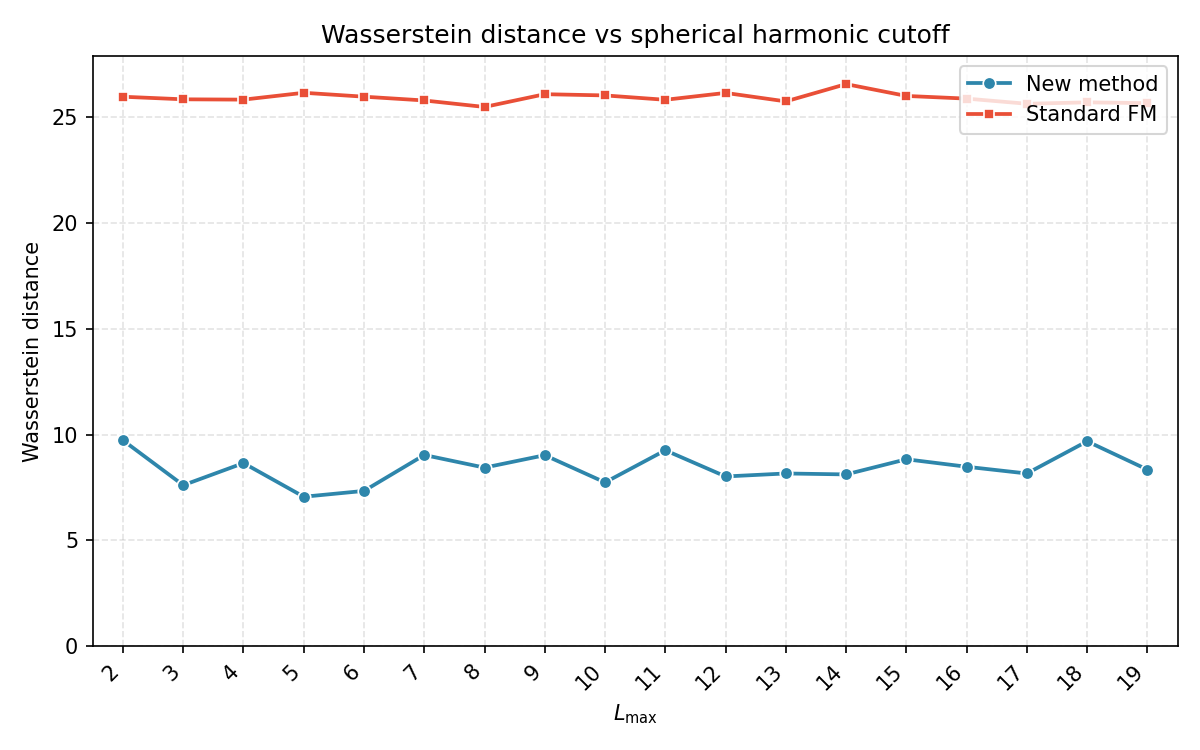
\includegraphics[width=\linewidth,height=0.78\textheight,keepaspectratio]{compare_wasserstein_runs.png}

  \vspace{0.1em}
  \scriptsize
  \textbf{Takeaway:} Standard FM $\approx 26$ (flat). Ours $\approx 7$--$10$; minimum $W_2 \approx 7.07$ at $L_{\max}{=}4$.
\end{frame}

\discussionframe{Experiment --- Wasserstein vs.\ \texorpdfstring{$L_{\max}$}{Lmax}}{
  \begin{itemize}
    \item Standard FM is \textbf{insensitive} to target band-limit --- wrong inductive bias, not wrong capacity.
    \item Our method tracks difficulty: higher $L_{\max}$ $\Rightarrow$ slightly higher $W_2$, with a sweet spot near $L_{\max}{=}4$.
    \item Non-monotonicity at 500 epochs may reflect under-convergence rather than true sensitivity.
  \end{itemize}
}

\begin{frame}{Experiment --- note on convergence}
  \small
  This sweep used \textbf{500 epochs} (vs.\ 1000 in the component-ablation run).

  \vspace{0.6em}
  The non-monotonic curve is likely \textbf{not the expected behavior} --- probably due to insufficient convergence at 500 epochs.

  \vspace{0.6em}
  Follow-up: epoch budget scaled to \textbf{1000} for the next $L_{\max}$ sweep.
\end{frame}

\begin{frame}{Experiment --- $L_{\max}$ sensitivity (1000 epochs)}
  \vspace{-0.55em}
  \centering
  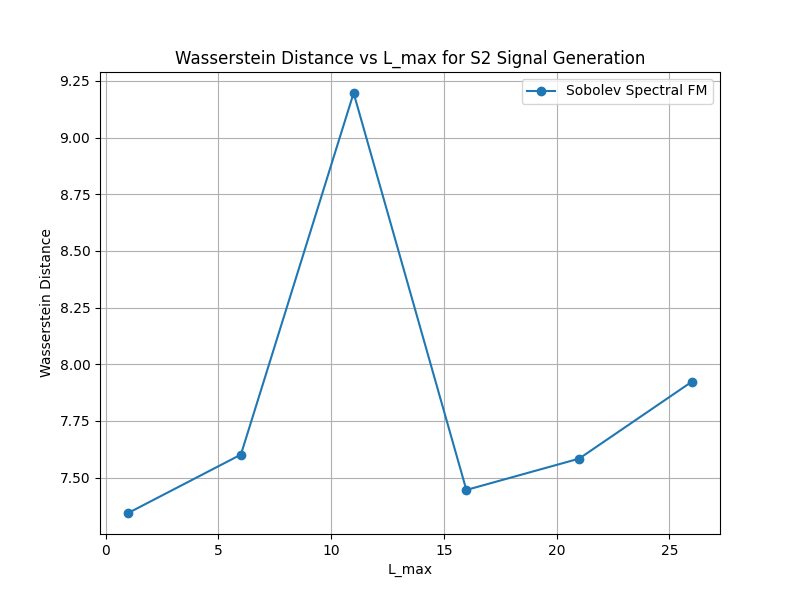
\includegraphics[width=\linewidth,height=0.88\textheight,keepaspectratio]{L_sensitivity.png}
\end{frame}

% ---------------------------------------------------------------------------
\section{Experiment: neural operator velocity field}

\begin{frame}
  \centering
  {\LARGE Architectures}
\end{frame}

\begin{frame}{Exploring other Neural operators}
  \begin{itemize}
    \item \texttt{fno2d} --- standard 2D Fourier Neural Operator (FFT on the grid)
    \item \texttt{laplacian\_fno} --- graph-Laplacian eigenbasis conv (NORM-style)
    \item \texttt{sobolev\_fno} --- same basis, with Sobolev whitening in encode/decode
  \end{itemize}
\end{frame}

\begin{frame}{Neural operator in flow matching}
  \textbf{Operator view.}\quad Treat the state as a function $a$ on $N$ nodes (grid cells or flattened atoms), not a single vector in $\mathbb{R}^N$:
  \[
    v_\theta \;=\; Q \circ \mathcal{L}_T \circ \cdots \circ \mathcal{L}_1 \circ P,
    \qquad
  \]
  \begin{itemize}\setlength{\itemsep}{0.15em}
    \item $P$ (\textbf{lift}): $(a, \text{coords}, t) \mapsto$ hidden channels $v \in \mathbb{R}^{C \times N}$
    \item $\mathcal{L}_\ell$ (\textbf{spectral layer}): integral kernel in a truncated basis + local $1{\times}1$ bypass
    \item $Q$ (\textbf{project}): hidden channels $\mapsto$ per-node velocity
  \end{itemize}

  \vspace{0.35em}
  \small
  FM interface unchanged: \texttt{forward(x, t)} with \texttt{x} $\in \mathbb{R}^{B \times N}$, \texttt{t} $\in \mathbb{R}^{B \times 1}$.
  Adapters in \texttt{models/FNO.py}, \texttt{models/manifold\_fno.py}.
\end{frame}

\begin{frame}{One spectral layer --- shared recipe}
  \small
  Every backbone layer has the same structure (FNO, Laplacian FNO, Sobolev FNO):
  \[
    v_{\ell+1} \;=\; \sigma\!\Bigl(
      \underbrace{\mathcal{D}^{-1}\!\bigl(R_\ell \cdot \mathcal{E}(v_\ell)\bigr)}_{\text{integral operator}}
      \;+\;
      \underbrace{W_\ell\, v_\ell}_{\text{local bypass}}
    \Bigr).
  \]

  \vspace{0.35em}
  \textbf{Encode} $\mathcal{E}$, \textbf{decode} $\mathcal{D}^{-1}$, learned mode weights $R_\ell$:

  \vspace{0.2em}
  \begin{table}
    \centering
    \begin{tabular}{@{}lll@{}}
      \toprule
      \textbf{Backbone} & $\mathcal{E}(v)$ & $R_\ell$ acts on \\
      \midrule
      \texttt{fno1d} / \texttt{fno2d} &
      $\mathrm{rfft}(v)$ / $\mathrm{rfft2}(v)$ &
      first $K$ Fourier modes \\
      \texttt{laplacian\_fno} &
      $\Phi^\top v$ &
      first $K$ Laplacian eigenmodes $\phi_k$ \\
      \texttt{sobolev\_fno} &
      $(1{+}\lambda_k)^{\alpha/2}\,\langle v,\phi_k\rangle$ &
      whitened coefficients (decode with inverse scale) \\
      \bottomrule
    \end{tabular}
  \end{table}

  \vspace{0.25em}
  \footnotesize
  \textbf{Note on \texttt{sobolev\_fno}:} weighting coefficients without changing the basis $\{\phi_k\}$ (scaling only) does not buy extra expressivity---encode and decode scales cancel within each layer, so it is equivalent to \texttt{laplacian\_fno}. Just a weird idea I wanted to try out.

  \normalsize
\end{frame}

\begin{frame}{\texorpdfstring{$S^2$}{S2} architecture comparison --- balanced capacity}
  \small
  Fair backbone comparison (\texttt{compare\_manifold\_fno\_s2}): matched trainable parameter count across backbones.

  \vspace{0.4em}
  \begin{table}
    \centering
    \begin{tabular}{@{}lr@{}}
      \toprule
      \textbf{Backbone} & \textbf{Parameters} \\
      \midrule
      \texttt{mlp} & 137{,}120 \\
      \texttt{fno2d} & 133{,}505 \\
      \texttt{laplacian\_fno} & 133{,}505 \\
      \texttt{sobolev\_fno} & 133{,}505 \\
      \bottomrule
    \end{tabular}
  \end{table}

  \vspace{0.35em}
  \normalsize
  Neural operators are within $\approx 3\%$ of the MLP --- differences in $W_2$ reflect architecture, not capacity.
\end{frame}

% ---------------------------------------------------------------------------
\section{Standard \texorpdfstring{$S^2$}{S2} spherical-harmonic signals}

\begin{frame}{Experiment --- standard \texorpdfstring{$S^2$}{S2} spherical harmonics signal}
  \footnotesize
  Balanced backbones ($\approx 137$k) on band-limited SH target ($L_{\max}{=}5$, $20{\times}40$ grid); \texttt{compare\_manifold\_fno\_s2}.

  \vspace{0.25em}
  \begin{table}
    \centering
    \scriptsize
    \setlength{\tabcolsep}{3.5pt}
    \begin{tabular}{@{}lccc@{}}
      \toprule
      \textbf{Backbone} &
      \textbf{Standard FM (1000 ep)} &
      \textbf{Spectral FM (500 ep)} &
      \textbf{Spectral FM (1000 ep)} \\
      \midrule
      \texttt{mlp} & 28.39 & 7.21 & 7.63 \\
      \texttt{fno2d} & \textbf{6.36} & 13.92 & 7.64 \\
      \texttt{laplacian\_fno} & 7.02 & 7.62 & \textbf{7.37} \\
      \texttt{sobolev\_fno} & 6.40 & 29.15 & 32.44 \\
      \bottomrule
    \end{tabular}
  \end{table}

  \vspace{0.1em}
  \scriptsize
  Standard FM: Gaussian source + MSE. Spectral FM: Mat\'ern + Laplacian spectral loss ($\alpha{=}{-}1$, $\beta{=}2$, $\nu{=}3$, $\tau{=}2$).

  \vspace{0.15em}
  \normalsize
  \textbf{Takeaway:} Injecting topological information (graph Laplacian / Fourier structure in the architecture) with standard FM reaches $W_2 \approx 6$--$7$, \textbf{slightly} beating our spectral FM ($\approx 7.4$). This SH-sampling task may be \textbf{biased} toward Fourier backbones (natural spherical basis); we need a less biased benchmark. Our spectral loss may also be \textbf{redundant or confusing} when target and backbone already share spectral geometry.
\end{frame}

% ---------------------------------------------------------------------------
\section{Experiment: AD3 molecular benchmark}

\begin{frame}
  \centering
  {\LARGE Molecular conformer generation}\\[0.5em]
  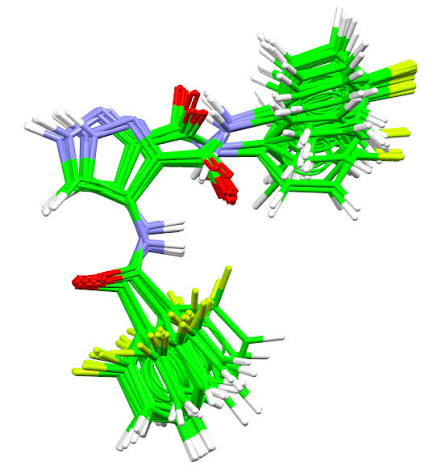
\includegraphics[width=0.48\linewidth,height=0.62\textheight,keepaspectratio]{conformer.jpeg}
\end{frame}

\begin{frame}{Molecular conformer generation --- task}
  \textbf{Goal:} learn a generative transport map from a simple prior to \textbf{equilibrium molecular conformations} sampled by MD.

  \vspace{0.5em}
  \begin{itemize}
    \item \textbf{Input / output:} 3D atomic coordinates $x \in \mathbb{R}^{N_{\mathrm{atoms}} \times 3}$
    \item \textbf{Our angle:} spectral / Sobolev flow matching with geometry-aware priors (as on $S^2$); graph Laplacian from \textbf{covalent bonds} or \textbf{heat-kernel} on interatomic distances
    \item \textbf{Evaluation:} distributional match of dihedral angles, energies, and structural observables
  \end{itemize}

  \vspace{0.4em}
  \small
  Reference baseline: \href{https://arxiv.org/abs/2302.01170}{Timewarp (NeurIPS 2023)} --- normalizing-flow MCMC for peptide acceleration.
\end{frame}

\begin{frame}{Alanine dipeptide --- the molecule}
  \begin{columns}[c,onlytextwidth]
    \column{0.42\textwidth}
    \centering
    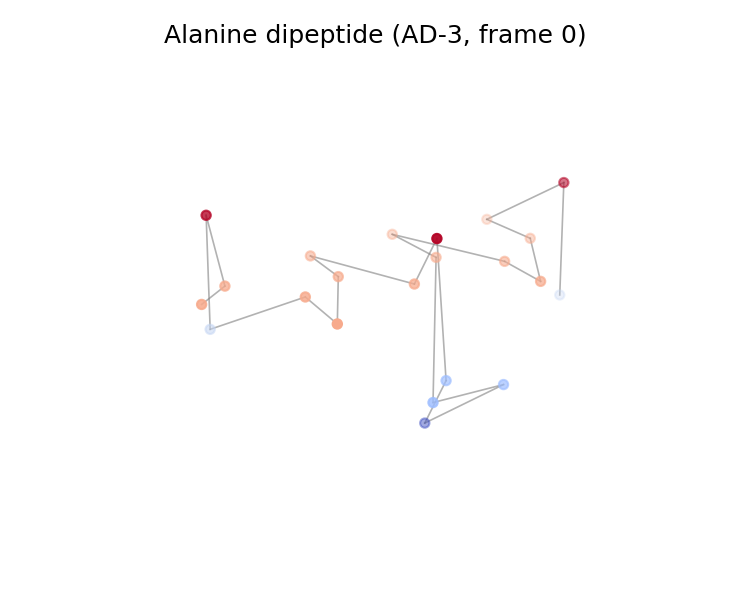
\includegraphics[width=\linewidth]{ad3_structure.png}\\[0.3em]
    {\scriptsize AD-3 initial frame (\texttt{ad1-traj-state0.pdb})}

    \column{0.54\textwidth}
    \textbf{Alanine dipeptide (AD)} --- smallest dipeptide:
    \begin{itemize}\setlength{\itemsep}{0.15em}
      \item 22 atoms (backbone + side chains)
      \item Standard benchmark in MD software and ML-for-chemistry
    \end{itemize}

    \vspace{0.4em}
    \small
    \href{https://huggingface.co/datasets/microsoft/timewarp}{microsoft/timewarp} dataset card, AD-3 folder.
  \end{columns}
\end{frame}

\begin{frame}{AD-3 dataset (Microsoft TimeWarp)}
  \small
  HuggingFace \texttt{AD-3/}: \texttt{train/ad1-traj-*} (long MD) and \texttt{test/ad2-traj-*} (held-out).

  \vspace{0.45em}
  Each split: \texttt{*-state0.pdb} + \texttt{*-arrays.npz} with \texttt{positions} $(T,22,3)$.

  \vspace{0.45em}
  Training trajectory: $8{\times}10^5$ frames (OpenMM, AMBER14, implicit solvent, $T{=}310$\,K).

  \vspace{0.45em}
  Reported experiments subsample $\mathcal{O}(10^3)$--$10^4$ training frames, not the full trajectory.
  \normalsize
\end{frame}

\begin{frame}{Evaluation metrics}
  \footnotesize
  Generated $\{x_i^{\mathrm{gen}}\}_{i=1}^{M}$, reference $\{x_j^{\mathrm{true}}\}_{j=1}^{M}$ (COM-relative coords, $x \in \mathbb{R}^{66}$).

  \vspace{0.3em}
  \textbf{Euclidean $W_2$}
  \[
    d_{\mathrm{Eucl}}^2(x,y)=\|x-y\|_2^2,\quad
    W_2=\sqrt{\min_{\pi\in\Pi(a,b)}\sum_{i,j}\pi_{ij}\,d_{\mathrm{Eucl}}^2(x_i^{\mathrm{gen}},x_j^{\mathrm{true}})},
  \]
  uniform weights $a_i=b_j=1/M$; exact EMD (\texttt{ot.emd2}).

  \vspace{0.25em}
  \textbf{Sobolev $W_2$} \quad ($\phi_k,\lambda_k$ from bond-graph / heat-kernel Laplacian; $\beta{=}2$ on AD-3)
  \[
    d_{\mathrm{Sob}}^2(x,y)=\sum_{k=1}^{K}(1+\lambda_k)^{-\beta}\langle\phi_k,x-y\rangle^2,\quad
    W_{2,\mathrm{Sob}}=\sqrt{\min_{\pi}\sum_{i,j}\pi_{ij}\,d_{\mathrm{Sob}}^2(x_i^{\mathrm{gen}},x_j^{\mathrm{true}})}.
  \]

  \vspace{0.25em}
  \textbf{COM-aligned RMSD} \quad reshape $x\to\{r_a\}_{a=1}^{22}\subset\mathbb{R}^3$, $\tilde{r}_a=r_a-\bar{r}$, $\bar{r}=\frac{1}{22}\sum_a r_a$,
  \[
    \mathrm{RMSD}(g,t)=\sqrt{\tfrac{1}{22}\sum_{a=1}^{22}\|\tilde{g}_a-\tilde{t}_a\|_2^2},\quad
    \overline{\mathrm{RMSD}}=\frac{1}{M}\sum_{i=1}^{M}\min_{j}\mathrm{RMSD}(g_i,t_j)\;\;(\text{nm}).
  \]
  \textit{Per-atom structural error after center-of-mass alignment; each generated conformer is matched to its closest reference.}
  \scriptsize
  \texttt{Tests/metrics.py} \quad Lower is better for all three.
\end{frame}

\begin{frame}{Experiment --- setup}
  \textbf{Conformer generation on AD-3} (alanine dipeptide, Microsoft TimeWarp)

  \vspace{0.5em}
  \begin{columns}[T,onlytextwidth]
    \column{0.48\textwidth}
    \textbf{Data \& representation}
    \begin{itemize}\setlength{\itemsep}{0.15em}
      \item Train: \texttt{ad1-traj} ($8{\times}10^5$ frames, subsample 8192)
      \item Test: \texttt{ad2-traj} (1024 held-out frames; final comparison also uses 2048)
      \item State: COM-relative coords, $22{\times}3 = 66$ dims
      \item Graph: covalent bond Laplacian (\texttt{molecule\_graph.py})
    \end{itemize}

    \column{0.48\textwidth}
    \textbf{Training}
    \begin{itemize}\setlength{\itemsep}{0.15em}
      \item MLP or balanced neural-operator backbones ($\approx 137$k params)
      \item FM steps: 8 \quad Epochs: 1000 \quad Batch: 512
      \item $\alpha{=}{-}1$, $\beta{=}2.0$, $\nu{=}3.0$, $\tau{=}2.0$
      \item Ours: Mat\'ern source + Laplacian spectral loss
    \end{itemize}
  \end{columns}
\end{frame}

\begin{frame}{Experiment --- standard vs.\ spectral FM (MLP)}
  \small
  Same MLP backbone (\texttt{intermediate\_dim=512}); only FM recipe differs.

  \vspace{0.35em}
  \begin{table}
    \centering
    \begin{tabular}{@{}lccc@{}}
      \toprule
      \textbf{Configuration} & \textbf{$W_2$ (Eucl.)} & \textbf{$W_2$ (Sob.)} & \textbf{RMSD mean (nm)} \\
      \midrule
      Standard FM (Gaussian source, MSE loss) & 0.868 & --- & 0.172 \\
      Ours (Mat\'ern source + spectral loss) & \textbf{0.671} & \textbf{0.522} & \textbf{0.126} \\
      \bottomrule
    \end{tabular}
  \end{table}

  \vspace{0.4em}
  \normalsize
  \textbf{Takeaway:} On real MD conformations, the $S^2$ recipe transfers --- spectral FM cuts Euclidean $W_2$ by $\approx 23\%$ and RMSD by $\approx 27\%$ vs.\ standard FM.
\end{frame}

\discussionframe{Experiment --- standard vs.\ spectral FM}{
  \begin{itemize}
    \item \textbf{Transfer to real data:} Mat\'ern prior + spectral loss helps beyond synthetic $S^2$ fields.
    \item Sobolev $W_2$ ($0.52$) is lower than Euclidean ($0.67$) --- metric aligns with smooth molecular graphs.
    \item COM-aligned RMSD $\approx 0.13$\,nm is chemically reasonable for a small peptide scaffold.
  \end{itemize}
}

\begin{frame}{Experiment --- architecture comparison (balanced capacity)}
  \footnotesize
  Fair comparison at $\approx 137$k trainable parameters per backbone; FM recipe varies by column.

  \vspace{0.25em}
  \begin{table}
    \centering
    \setlength{\tabcolsep}{3.5pt}
    \begin{tabular}{@{}l cc ccc@{}}
      \toprule
      & \multicolumn{2}{c}{\textbf{Standard FM}} & \multicolumn{3}{c}{\textbf{Spectral FM (ours)}} \\
      \cmidrule(lr){2-3} \cmidrule(lr){4-6}
      \textbf{Backbone} &
      \textbf{$W_2$} & \textbf{RMSD} &
      \textbf{$W_2$} & \textbf{$W_2^{\mathrm{Sob}}$} & \textbf{RMSD} \\
      \midrule
      \texttt{fno1d} &
      1.340 & \textbf{0.167} &
      \textbf{0.753} & \textbf{0.624} & \textbf{0.114} \\
      \texttt{mlp} &
      \textbf{1.015} & 0.206 &
      0.815 & 0.662 & 0.146 \\
      \texttt{graph\_laplacian\_fno} &
      1.382 & 0.188 &
      0.944 & 0.751 & 0.159 \\
      \texttt{graph\_sobolev\_fno} &
      1.336 & 0.177 &
      1.202 & 0.986 & 0.185 \\
      \bottomrule
    \end{tabular}
  \end{table}

  \vspace{0.25em}
  \scriptsize
  Standard FM: Gaussian source + MSE loss.
  Spectral FM: Mat\'ern source + Laplacian spectral loss.

  \vspace{0.2em}
  \normalsize
  \textbf{Takeaway:} Spectral FM improves every backbone ($W_2$ $\downarrow$ $25$--$44\%$, RMSD $\downarrow$ $18$--$32\%$); \texttt{fno1d} best overall under our recipe.
  \textit{\scriptsize Likely reason: \texttt{fno1d} works in Fourier space, where convolution is diagonal---a natural match for learning spectrally structured velocity fields.}
\end{frame}

\begin{frame}
  \centering
  {\LARGE Different graph Laplacians representing the molecule}
\end{frame}

\begin{frame}{Experiment --- heat-kernel graph Laplacian}
  \textbf{Motivation:} replace covalent bonds with a \textbf{geometry-aware} graph from 3D distances.

  \vspace{0.5em}
  Edge weights from Euclidean interatomic distance (reference PDB frame):
  \[
    w_{ij} = \exp\!\left(-\frac{d_{ij}^2}{2\sigma^2}\right),
    \qquad
    L = D - W,
  \]
  with $\sigma$ defaulting to the \textbf{median pair distance} among included atoms (\texttt{graph\_type="heat"} in \texttt{molecule\_graph.py}).

  \vspace{0.4em}
  Same spectral FM recipe (Mat\'ern source + Laplacian spectral loss); compare \texttt{graph\_type="heat"} vs.\ \texttt{"bond"} at matched 1000-epoch budget (final results on next slide).
\end{frame}

\begin{frame}{Experiment --- heat vs.\ bond graph (final comparison)}
  \tiny
  Matched setup: 1000 epochs, 16384 train frames, batch 1024, 2048 test, 8 FM steps.

  \vspace{0.15em}
  \begin{table}
    \centering
    \setlength{\tabcolsep}{2pt}
    \begin{tabular}{@{}l ccc ccc cc cc@{}}
      \toprule
      & \multicolumn{3}{c}{\textbf{Spectral FM (heat)}} &
        \multicolumn{3}{c}{\textbf{Spectral FM (bond)}} &
        \multicolumn{2}{c}{\textbf{Standard FM (bond)}} &
        \multicolumn{2}{c}{\textbf{Standard FM (heat)}} \\
      \cmidrule(lr){2-4} \cmidrule(lr){5-7} \cmidrule(lr){8-9} \cmidrule(lr){10-11}
      \textbf{Backbone} &
      $W_2$ & RMSD & $W_2^{\mathrm{Sob}}$ &
      $W_2$ & RMSD & $W_2^{\mathrm{Sob}}$ &
      $W_2$ & RMSD &
      $W_2$ & RMSD \\
      \midrule
      \texttt{mlp} &
      1.24 & 0.236 & 0.14 &
      0.72 & 0.139 & \textbf{0.57} &
      \textbf{0.90} & \textbf{0.184} & \textbf{0.90} & 0.185 \\
      \texttt{fno1d} &
      \textbf{1.08} & \textbf{0.117} & 0.38 &
      \textbf{\underline{0.70}} & \textbf{\underline{0.107}} & 0.58 &
      1.27 & 0.155 & 1.29 & \textbf{0.158} \\
      \texttt{graph\_laplacian\_fno} &
      1.21 & 0.203 & \textbf{0.11} &
      1.12 & 0.197 & 0.88 &
      1.38 & 0.193 & 1.29 & 0.173 \\
      \texttt{graph\_sobolev\_fno} &
      1.23 & 0.189 & 0.12 &
      0.95 & 0.151 & 0.76 &
      1.36 & 0.186 & 1.28 & 0.168 \\
      \bottomrule
    \end{tabular}
  \end{table}

  \vspace{0.15em}
  \scriptsize
  Spectral FM: Mat\'ern source + Laplacian spectral loss. Standard FM: Gaussian source + MSE.
  Bold = best per column; underline = best overall Euclidean $W_2$ / RMSD.
  For Standard FM, bond vs.\ heat only enters via the Laplacian in \texttt{graph\_laplacian\_fno} / \texttt{graph\_sobolev\_fno} (\texttt{mlp}, \texttt{fno1d} unchanged).

  \vspace{0.15em}
  \normalsize
  \textbf{Takeaway:} Bond graph wins on Euclidean $W_2$/RMSD under spectral FM (\texttt{fno1d} best: $W_2{=}0.70$, RMSD $0.11$\,nm). Heat graph yields very low Sobolev $W_2$ ($\approx 0.11$--$0.14$) but worse Cartesian fit.
\end{frame}

\begin{frame}{Experiment --- discussion \& open questions}
  \begin{itemize}
    \item \textbf{Confirmed:} Mat\'ern + spectral loss helps on real molecular data, not only synthetic $S^2$ fields.
    \item \textbf{Best backbone so far:} \texttt{fno1d} (RMSD $\approx 0.11$\,nm); MLP competitive.
    \item \textbf{Still open:} Ramachandran / basin-occupancy histograms vs.\ MD (not yet plotted).
  \end{itemize}
\end{frame}

% ---------------------------------------------------------------------------
\section{Summary}

\begin{frame}{Summary \& next steps}
  \begin{itemize}
    \item Synthetic $S^2$ fields provide a controlled sanity check before harder real data.
    \item Component ablation: Mat\'ern + spectral loss best ($W_2 \approx 7.98$); Mat\'ern source is the dominant ingredient.
    \item Standard $S^2$ SH signal: under standard FM, \texttt{fno2d} best ($W_2 \approx 6.4$); under spectral FM, all except \texttt{sobolev\_fno} $\approx 7.4$ at 1000 epochs.
    \item AD-3 conformers: spectral FM beats standard ($W_2$ 0.67 vs.\ 0.87; RMSD 0.13 vs.\ 0.17\,nm); \texttt{fno1d} best among balanced backbones.
    \item Heat vs.\ bond graph (1000 epochs): bond + spectral FM best on Euclidean $W_2$/RMSD (\texttt{fno1d} $0.70$ / $0.11$\,nm); heat graph yields Sobolev $W_2 \approx 0.11$--$0.14$ at the cost of Cartesian fit.
    \item Still open: Ramachandran evaluation on AD-3.
  \end{itemize}
\end{frame}

% ---------------------------------------------------------------------------
\section{Theory: why Mat\'ern + Sobolev loss?}

\begin{frame}{Theory --- spectral setup}
  \small
  On the grid Laplacian $L$ with eigenpairs $(\lambda_k, \phi_k)$, our method lives in a \textbf{Sobolev-weighted} space:
  \[
    \|f\|_{H^\alpha}^2 = \sum_k (1+\lambda_k)^{\alpha}\, |\langle f, \phi_k\rangle|^2 .
  \]

  \vspace{0.35em}
  Three ingredients (component ablation):
  \begin{itemize}\setlength{\itemsep}{0.15em}
    \item \textbf{Mat\'ern source} --- prior at $t{=}0$: $x_0 \sim \mathcal{N}\bigl(0, (\tau I + L)^{-\nu}\bigr)$
    \item \textbf{Sobolev (spectral) loss} --- CFM residual weighted by $(1+\lambda_k)^{\alpha}$ in \texttt{SpectralFM}
    \item \textbf{Target} --- band-limited SH field with $\mathrm{Var}(\xi_{\ell m}) \propto \bigl(\ell(\ell{+}1)\bigr)^{-s/2}$
  \end{itemize}

  \vspace{0.35em}
  \textbf{Empirical fact:} Mat\'ern alone ($W_2 \approx 26$) and spectral loss alone ($W_2 \approx 25$) match standard FM; \textbf{both together} $\approx 7.98$.
\end{frame}

\begin{frame}{Theory --- Mat\'ern source alone fails}
  \small
  Mat\'ern fixes \textbf{where you start}; standard $L^2$ loss trains in the \textbf{wrong metric}.

  \vspace{0.35em}
  \textbf{1.\ Prior is correct, objective is not.}\quad
  $\mathrm{Var}(\langle x_0, \phi_k\rangle) = (\tau + \lambda_k)^{-\nu}$, but CFM minimizes
  \[
    \mathcal{L} = \mathbb{E}\,\|v_\theta(t, x_t) - v^\star\|_{\mathbb{R}^d}^2
  \]
  over \textbf{grid coordinates}, not Laplacian modes. High-frequency mesh directions dominate the $L^2$ norm of the velocity residual even when $x_0, x_1$ are smooth.

  \vspace{0.35em}
  \textbf{2.\ Transport stays hard in ambient $\mathbb{R}^d$.}\quad
  Mat\'ern $\mu_0$ and smooth target $\mu_1$ are close in $H^\alpha$, but $L^2$ training optimizes a flat Euclidean flow. Correct boundary condition, wrong inner product --- the learned ODE does not converge to the geometrically correct map.

  \vspace{0.25em}
  \textit{Mat\'ern $\Rightarrow \mu_0 \in \mathcal{H}^s$; $L^2$ CFM optimizes in $L^2(\text{grid})$ --- different topologies.}
\end{frame}

\begin{frame}{Theory --- Sobolev loss alone fails}
  \small
  Sobolev loss fixes \textbf{how you train}; Gaussian source leaves \textbf{where you start} wrong.

  \vspace{0.35em}
  \textbf{1.\ White source vs.\ smooth target.}\quad
  $x_0 \sim \mathcal{N}(0,I)$ gives $\mathrm{Var}(\langle x_0, \phi_k\rangle) = 1$ for all $k$, while target variance decays as $\lambda_k^{-s}$. For large $\lambda_k$, white noise has orders of magnitude more high-frequency energy than the target, so
  \[
    x_1 - x_0 \approx x_1 - \text{(large HF noise)} .
  \]

  \vspace{0.35em}
  \textbf{2.\ Reweighting $\neq$ fixing the initial measure.}\quad
  With $\alpha = -1$, the loss downweights high $\lambda_k$, but at inference we still integrate from fresh $\mathcal{N}(0,I)$ samples. The marginal pushforward at $t{=}0$ remains the wrong measure on the manifold.

  \vspace{0.35em}
  \textbf{3.\ RKHS view.}\quad
  Any map from isotropic Gaussian to a smooth GP must create large Cameron--Martin norm (highly oscillatory trajectories). Downweighting those modes in the loss does not make white noise a good prior.
\end{frame}

\begin{frame}{Theory --- why both together work}
  \small
  The two components are \textbf{dual} with respect to the same operator $L$:
  \[
    \boxed{
      \text{Prior: } C_0 = (\tau I + L)^{-\nu}
      \quad\longleftrightarrow\quad
      \text{Metric: } \|\cdot\|_{H^\alpha},\;\; \alpha < 0
    }
  \]

  \vspace{0.35em}
  With $\nu{=}3$, $\tau{=}2$, $\alpha{=}{-}1$, $s{=}2$ (component ablation):
  \begin{itemize}\setlength{\itemsep}{0.12em}
    \item \textbf{Aligned endpoints} --- $x_0$ and $x_1$ are smooth fields with comparable spectral decay; $x_1 - x_0$ is a small structured perturbation in $H^\alpha$, not ``smooth minus white noise.''
    \item \textbf{Matched geometry} --- Sobolev loss trains the vector field in the same norm where $\mu_0$ and $\mu_1$ are close (approx.\ Sobolev OT between compatible GPs).
    \item \textbf{Band-diagonal CFM} --- low $\lambda_k$ modes carry transport; high $\lambda_k$ modes have tiny variance \emph{and} tiny loss weight.
  \end{itemize}

  \vspace{0.25em}
  \textit{Kernel-methods principle: prior and regularizer must share the same kernel --- both built from $L$.}
\end{frame}

\begin{frame}{Theory --- Bayesian reading \& corollaries}
  \small
  \textbf{Bayesian view.}
  \begin{itemize}\setlength{\itemsep}{0.12em}
    \item Mat\'ern source $=$ \textbf{prior} on the function space
    \item Sobolev loss $=$ \textbf{likelihood / regularization} in the same space
    \item Using only one is inference with the right prior but wrong likelihood, or vice versa
  \end{itemize}

  \vspace{0.35em}
  \textbf{Why Sobolev OT adds little} ($7.98$ vs.\ $8.14$): once source and loss are aligned, random $(x_0, x_1)$ pairs are already reasonable in $H^\beta$; OT mainly helps when endpoints are spectrally mismatched.

  \vspace{0.35em}
  \textbf{Prior calibration:} choose $(\nu, \tau)$ so that $(\tau + \lambda_k)^{-\nu} \approx \lambda_k^{-s}$ on modes that carry target mass --- $(\nu, \tau, \alpha)$ are one geometric specification, not independent knobs.

  \vspace{0.35em}
  \textbf{One-line summary:} Mat\'ern aligns the initial measure with the manifold; Sobolev loss aligns the training metric with the same manifold. Either fix alone leaves a prior--metric mismatch; both together make CFM approximate Sobolev transport between two compatible Gaussian measures.
\end{frame}

\end{document}
